 \section{Possible Installation Troubleshootings}

We will try to help to fix the problems you may encounter during the installation. For that we will explain the role of each important files you got once you decompressed the archive.


To run the environment provided with this book or \sq, four files are necessary. We describe them now as we will use their name to help solve the possible problems you may encounter. 

The four files are: 
\begin{itemize}
\item The file named \ct{ReadyToUse.image}, called simply the \textbf{image}\index{image file} file and the file named \textbf{ReadyToUse.changes}, called simply the \textbf{changes} \index{changes files}file contain the information of your current system. These two files are synchronized by \sq automatically and \emph{should be writable}. Each time you save you environment they are synchronized. You should not edit then with another file editor or changes the name of the file manually. If you want to have different names, just use the \menu{save as ...}
menu item of the World menu (see~\ref{cha:Tour}), \sq will then create a new pair of files for you. 

 
\item The file named \ct{SqueakV3.sources}, also called \textbf{sources}\index{sources file} file contains the source of a part of the \sq environment. Do not try to edit manually, \sq accesses this file for you via its programming tools. This file should normally be always in the directory in which the image is.
  
\item The application \macvm for mac or \pcvm for PC is the \sq system. This is this application that runs when you program in \sq. It should then be executable. 
We refer to this file as the \index{Squeak application}\textbf{Squeak application}. In computer scientist jargon, this application is called a \index{virtual machine} virtual machine called or  a VM \index{VM} in short. 
\end{itemize}


As we already mentioned it the \textit{image} and \textit{changes} files should be writable. Certain operating systems change the properties of the files to read-only when copied from a CD. In such a case, \sq warns you with a message as shown in Figure~\ref{fig:readonlyfile}. If you get this message, simply quit \sq without saving (See section~\ref{}), change the property of the file to be writable and restart.  

\begin{figure}[!h]\centerline{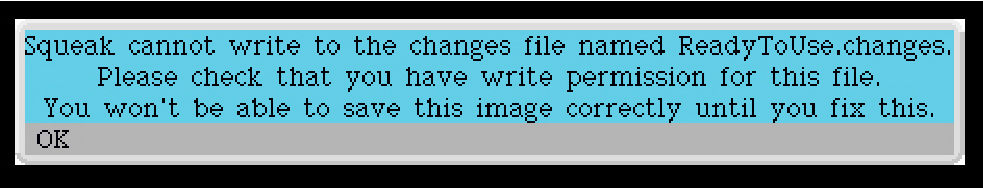
\includegraphics[width=\linewidth]{changesNotWritable}}\caption{The error message showing that
 the image (\ct{ReadyToUse.image}) or changes (\ct{ReadyToUse.changes}) files are not writable.\label{fig:readonlyfile}}
\end{figure}

Another possible problem you may encounter is related to the sources file named \ct{SqueakV3.sources}, this file or an alias to this file should be present in the directory where the image file is. When this file is not present you may get on Mac the first message shown in Figure~\ref{fig:sourcesMissing} (note that this message is not clear and refers to a problem related to aliases that is fixed in the current version of \sq) or the second message. To cure this problem, create an alias to the source file (\ct{SqueakV3.sources}) into the directory containing  your image or simply copy the sources file  to be in the same directory that the image file.

\begin{figure}[!h]\center{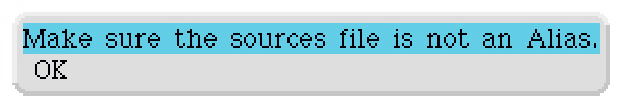
\includegraphics{sourcesMissing}}
\center{\includegraphics[width=\linewidth]{sourcesMissing2}}\caption{Some possible error messages indicating that the \textit{source} file (\ct{SqueakV3.sources}) is missing in the directory containing the \textit{image} file .\label{fig:sourcesMissing}}
\end{figure}


%%%%%%%%%%%%%%%%%%%%%%%%%%%%%%%%%%%%%%%%%%%
\summa

\begin{itemize}
\item To start the environment. 
Drag and drop the file terminating with the .image extension into the squeak application.
\item To interact with a turtle. Click on it, type expressions and hit the return key.
\end{itemize}